\begin{frame}{In queste diapositive}
\protect\hypertarget{in-queste-diapositive}{}

\begin{itemize}
\item
  Esercizio 4
\item
  Esercizio 1
\item
  Esercizio 9
\item
  Esercizio 10
\item
  Esercizio 11
\end{itemize}

\end{frame}

\begin{frame}{Esercizio 4}
\protect\hypertarget{esercizio-4}{}

Qual è l'effetto di breve periodo sul tasso di cambio di un aumento del
livello del PNL in termini reali, date le aspettative sul tasso di
cambio?


\end{frame}

\ifshowsolution

\begin{frame}{Soluzione esercizio 4}
\protect\hypertarget{soluzione-esercizio-4}{}

\begin{itemize}
\item
  aumenta la domanda di moneta in termini reali
\item
  le famiglie vorrebbero vendere titoli
\item
  le unità in deficit offrono un tasso di interesse più alto
\item
  un maggiore tasso di interesse nazionale fa

  \begin{itemize}
  \item
    aumentare la domanda di titoli nazionali da parte dei non residenti
    e la domanda di valuta nazionale
  \item
    diminuire la domanda di titoli stranieri da parte dei residenti:
    diminuire la domanda ti valuta estera
  \end{itemize}
\item
  il tasso di cambio si apprezza
\end{itemize}

\end{frame}

\begin{frame}{Rappresentazione grafica esercizio 4}
\protect\hypertarget{rappresentazione-grafica-esercizio-4}{}

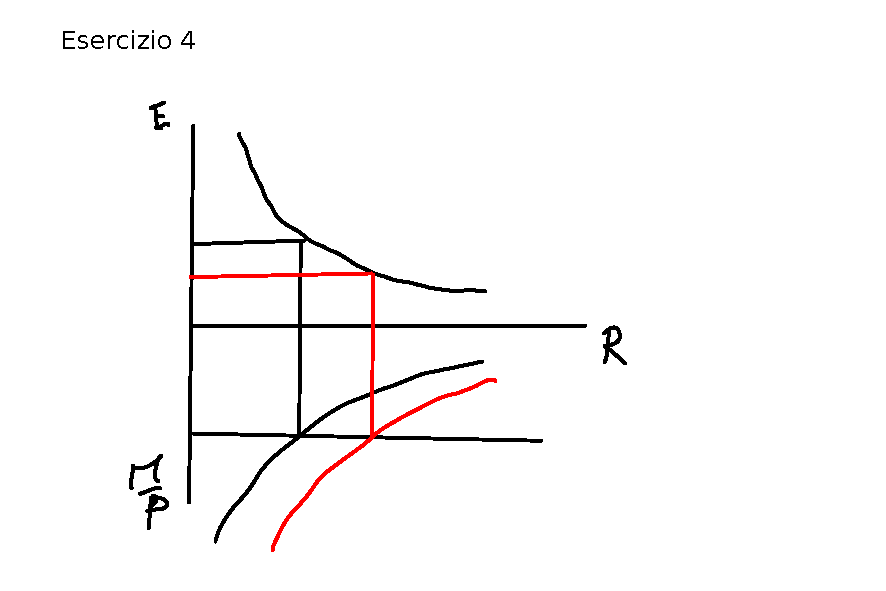
\includegraphics[scale=0.7]{pg_0003.pdf}


\end{frame}

\fi

\begin{frame}{Esercizio 1}
\protect\hypertarget{esercizio-1}{}

Supponete che vi sia una riduzione della domanda reale aggregata di
moneta e cioè uno spostamento negativo della funzione di domanda reale
aggregata di moneta. Illustrate gli effetti di breve e di lungo periodo
sul tasso di cambio, sul tasso di interesse e sul livello dei prezzi.

\end{frame}

\ifshowsolution

\begin{frame}{Soluzione esercio 1 breve periodo}
\protect\hypertarget{soluzione-esercio-1-breve-periodo}{}

\begin{itemize}
\item
  Nel breve periodo si attivano i seguenti meccanismi

  \begin{itemize}
  \item
    i sogetti desiderano detenere meno moneta
  \item
    la domanda di titoli aumenta
  \item
    le unità in deficit, vedendo molti acquirenti per i loro titoli,
    possono abbassare il tasso di interesse (\(R\downarrow\))
  \item
    \(R\downarrow \ \Rightarrow\) diminuzione della domanda di titoli
    nazionali da parte di non residenti

    \begin{itemize}
     
    \item
      la domanda della nostra valuta da parte di non residenti
      diminuisce
    \end{itemize}
  \item
    \(R\downarrow \ \Rightarrow\) aumento della domanda di titoli
    stranieri da parte di residenti

    \begin{itemize}
     
    \item
      la domanda della valuta straniera da parte dei residenti aumenta
    \end{itemize}
  \item
    Il tasso di cambio si deprezza (\(E \uparrow\))
  \end{itemize}
\end{itemize}

\end{frame}

\begin{frame}{Rappresetazione grafica breve periodo}
\protect\hypertarget{rappresetazione-grafica-breve-periodo}{}

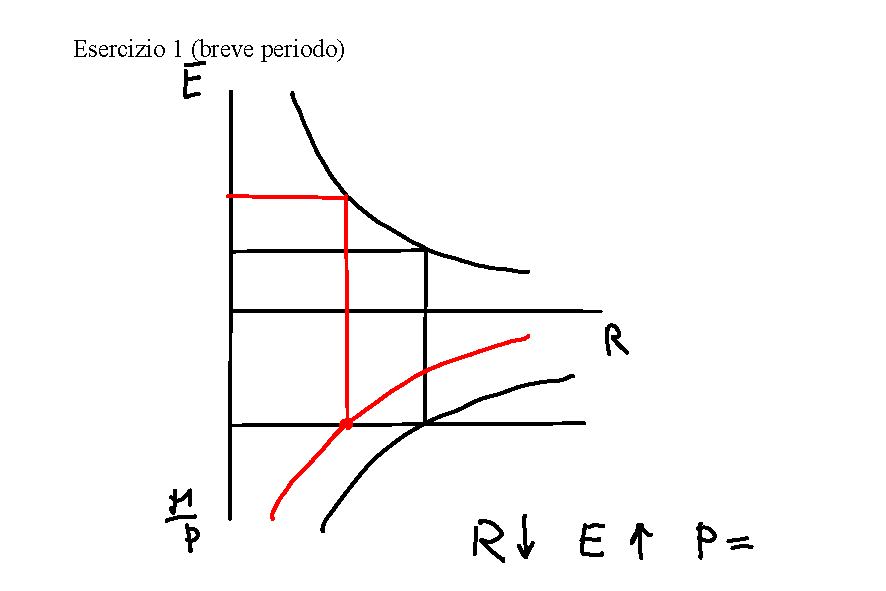
\includegraphics[scale=0.7]{pg_0001.pdf}

\end{frame}



\begin{frame}{Solizione esercizio 1 lungo periodo}
\protect\hypertarget{solizione-esercizio-1-lungo-periodo}{}

\begin{itemize}
\item
  la domanda di beni nazionali aumente per

  \begin{itemize}
  \item
    aumento della domanda dei non residenti per il deprezzamento di E
  \item
    aumento della domanda di investimenti per R basso
  \end{itemize}
\item
  ma non può variare perché di pieno impiego
\item
  i prezzi iniziano a salire
\item
  la quantità di moneta reale diminuisce
\item
  R e E ritornano ai loro livelli
\end{itemize}

\end{frame}

\begin{frame}{Rappresetazione grafica lungo periodo}
\protect\hypertarget{rappresetazione-grafica-lungo-periodo}{}

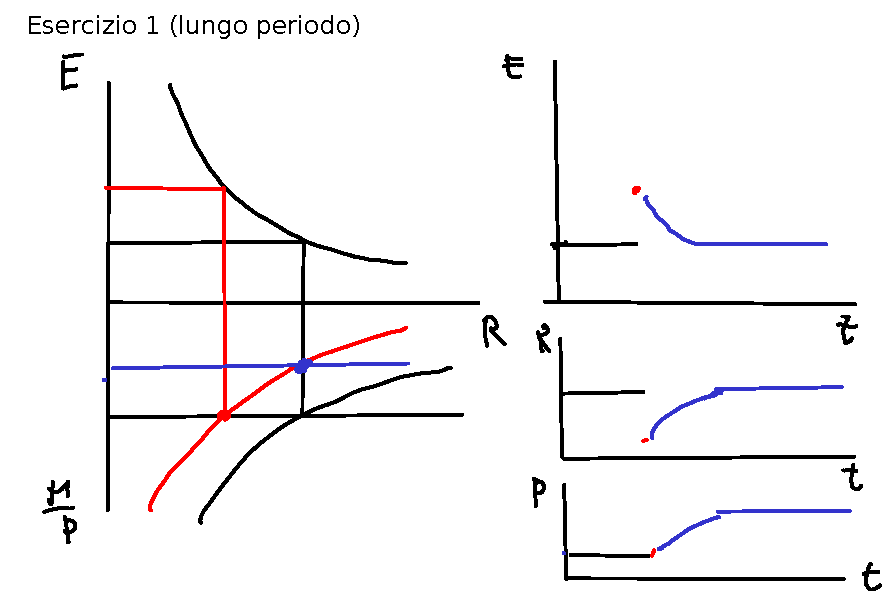
\includegraphics[scale=0.7]{pg_0002.pdf}

\end{frame}
\fi

\begin{frame}{Esercizio 9}
\protect\hypertarget{esercizio-9}{}

Nella nostra discussione sull'overshooting del tasso di cambio di breve
periodo, abbiamo supposto che la produzione reale fosse data. Assumiamo
invece che nel breve periodo un incremento dell'offerta di moneta
accresca il livello di produzione reale (un'ipotesi che sarà
giustificata nel Capitolo 6). In che modo questo fatto influisce
sull'iper-reazione del tasso di cambio data dall'aumento dell'offerta di
moneta? È possibile che il tasso di cambio evidenzi un undershooting?

\end{frame}

\ifshowsolution

\begin{frame}{Soluzione esercizio 9}
\protect\hypertarget{soluzione-esercizio-9}{}

\begin{itemize}
\item
  Il reddito può aumentare nel breve periodo, ma deve ritornare
  gradualmente al livello di pieno impiego
\item
  La domanda reale di moneta subisce uno spostamento verso destra
  iniziale, seguito da graduali spostamenti verso sinistra
\item
  l'offerta di moneta reale ha la stessa dinamica, uno spostamento verso
  destra a causa dell'aumento di \(M^s\), seguito da spostamenti
  graduali verso sinistra
\end{itemize}

\end{frame}

\begin{frame}{}
\protect\hypertarget{section}{}

\begin{itemize}
\item
  Se ci poniamo nella situazione ideale in cui la domanda e l'offerta di
  moneta si muovono ogni volta dello stesso ammontare, il tasso di
  interesse nazionale rimarrà costante.
\item
  la linea della parità dei tassi di interesse si sposta verso l'alto a
  causa dell'aumento del tasso di cambio atteso
\item
  In questo caso non si avrà overshooting.
\end{itemize}

\end{frame}

\fi

\begin{frame}{Esercizio 10}
\protect\hypertarget{esercizio-10}{}

La Figura 3.2 mostra che il tasso di interesse a breve in Giappone ha
attraversato periodi in cui è stato prossimo o addirittura uguale a
zero. Il fatto che i tassi di interesse in yen riportati nella figura
non siano mai diventati negativi è solo una coincidenza, o riuscite a
trovare qualche spiegazione del perché i tassi di interesse sono
vincolati dal basso al valore zero?

\end{frame}

\ifshowsolution

\begin{frame}{Soluzione esercizio 10}
\protect\hypertarget{soluzione-esercizio-10}{}

\begin{itemize}
\item
  Il tasso di rendimento della moneta rappresenta l'alternativa a quello
  dei titoli
\item
  il rendimento della moneta è uguale al tasso di inflazione cambiato di
  segno (deflazione: \(-\pi\))
\item
  il rendimento dei titoli (\(r=R-\pi\)) non può dunque scendere al di
  sotto del tasso di deflazione
  \[R-\pi\ge -\pi \qquad \Rightarrow \qquad R\ge 0\]
\end{itemize}

\end{frame}

\fi

\begin{frame}{Esercizio 11}
\protect\hypertarget{esercizio-11}{}

In che modo un tasso di interesse pari a zero potrebbe complicare il
compito della politica monetaria?

\end{frame}

\ifshowsolution

\begin{frame}{Soluzione esercizio 11}
\protect\hypertarget{soluzione-esercizio-11}{}

\begin{itemize}
\item
  L'aumento della quantità di moneta non ha effetto sui tassi di
  interesse
\item
  la ripresa dell'economia non può passare attraverso un aumento delgi
  investimenti
\end{itemize}

\end{frame}
\fi
